\section{Consequenties van de Lorentztransformatie}\label{CLT}

%%%%%%%%%%%
\subsection{Lat}
$S'$ beweegt met snelheid $v$ langs de $x$-as van $S$, dus gelden de Lorentztransformaties tussen $x$, $t$, $x'$ en $t'$: 
\begin{displaymath}
   x = \gamma (x' + \beta ct') 
\end{displaymath}
\begin{displaymath}
  ct = \gamma (ct' + \beta x').
\end{displaymath}
In  $S'$  ligt een lat, tussen $x' = 0$ (begin) en $x' = l$ (eind) .
De lat beweegt dus ook met snelheid $v$ door $S$.
\begin{itemize}
\item [a.]
  Je  bepaalt met de Lorentztransformatie de $x$-waarden van begin en eind 
van de lat als de (met de lat meebewegende) $S'$-klokken op nul staan, 
dus op $t' = 0$. Welke lengte vind je dan?
\item [b.]
  Wat zijn de $x$-waarden van begin en eind als de passerende $S$-klokken 
op nul staan, dus op $t = 0$?
\item [c.]
  Hoe groot is de lengte van de lat, als gezien in stelsel $S'$, en hoe groot is 
de lengte van de lat, als gezien in stelsel $S$?
\end{itemize}

%%%%%%%%%%%
%\subsection{Klok}
%Nu een klok die op een vaste plaats in $S'$ (op $x' = 0$) door $S$ beweegt.
%\begin{itemize}
%\item [a.]
%  Als  de klok zelf een tijdsverloop van 0 tot $T$ aangeeft, op welke plaats 
%bevindt hij zich dan in $S$ en welke tijd wijst een $S$-klok daar aan?
%\item [b.]
%  Toen de klok op nul stond passeerde hij juist een $S$-klok (in $x = 0$) 
%die ook op nul stond. 
%  Wat wijst die $S$-klok volgens waarnemers in $S'$ aan, als hun $S'$-klokken 
%op T staan?
%\item [c.]
%  Uit  welke  van  de  twee uitkomsten, a) of b), volgt de "tijddilatatie" 
%van de bewegende $S'$-klok?
%\item [d.]
%  Volgens de waarnemers in $S'$ was het de $S$-klok in $x = 0$ die bewoog. 
%Vertoont die volgens hen ook tijddilatatie?
%\end{itemize}

%%%%%%%%%
\subsection{Vier klokken}
Stelsel $S'$ beweegt t.o.v. stelsel $S$ met snelheid $v$ in de richting
van de positieve $x$-as.
Klok $A$ staat in de oorsprong van $S$ en klok $B$ in de oorsprong van $S'$.

% \begin{figure}
% \begin{center}
% \mbox{\epsfxsize=12cm\epsffile{oefeningen.pictures/klokken.eps}}
% \caption{Klokken}
% \label{f:klokken}
% \end{center}
% \end{figure}

\begin{figure}[ht]
\centering
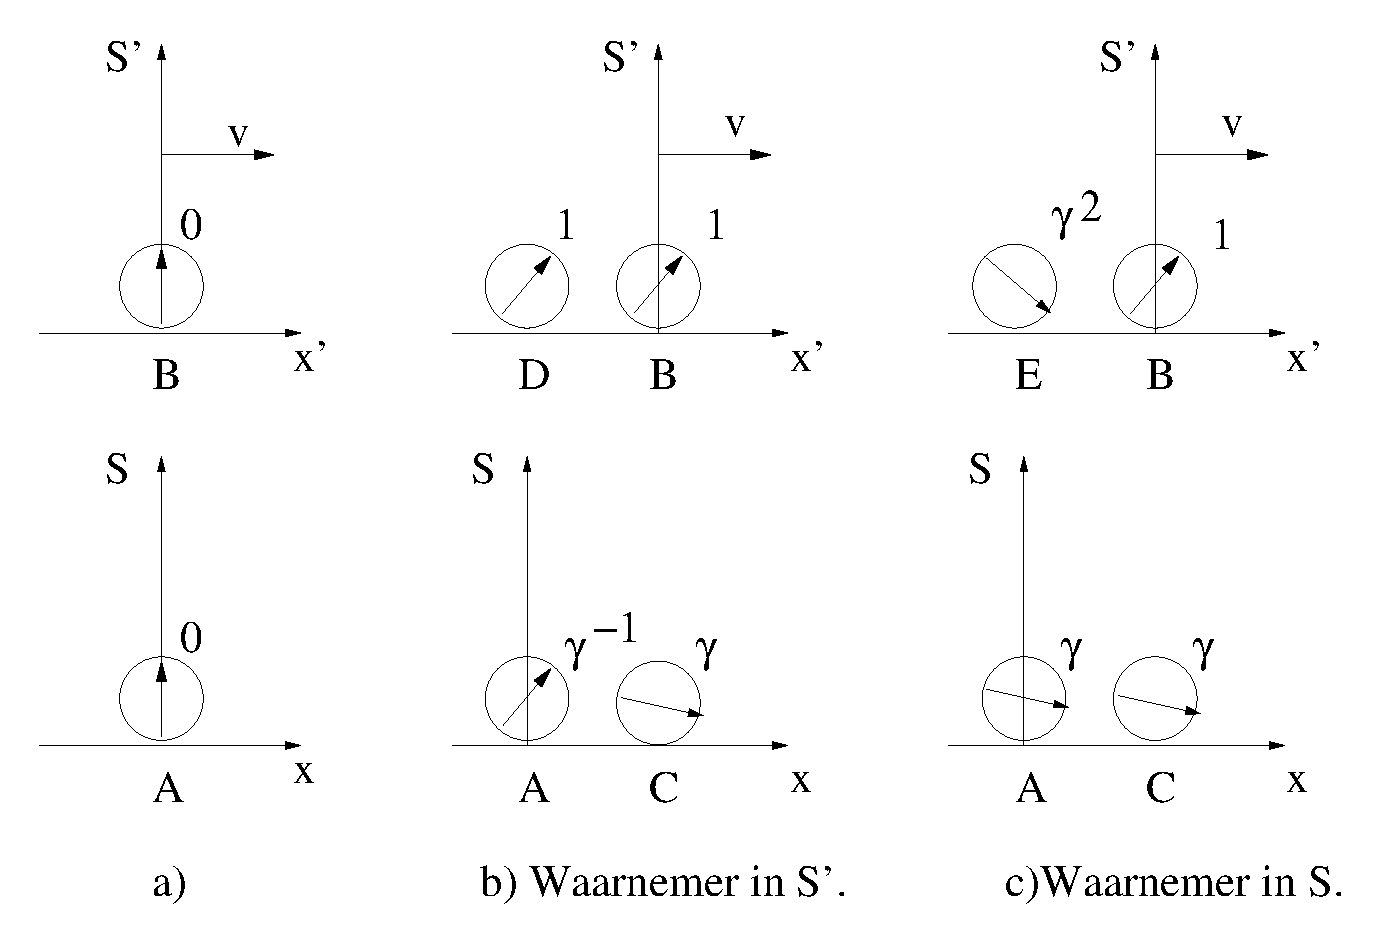
\includegraphics[width=.8\textwidth]{oefeningen.pictures/klokken}
\caption{Klokken}
\label{f:klokken}
\end{figure}

Als klok $B$ klok $A$ passeert staan ze beide op 0: $ct'=0$ en $ct=0$
(zie figuur \ref{f:klokken}a).


Even later, als klok $B$ op $ct'=1$ staat, passeert hij klok $C$ in $S$,
die dan op $ct=\gamma$ staat (zie fig. \ref{f:klokken}b).Volgens een waarnemer in $S'$ staat klok $A$ dan op $ct = \gamma^{-1}$ en 
passeert hij klok $D$ in $S'$, die dan op $ct'=1$ staat 
(fig. \ref{f:klokken}b). Volgens een waarnemer in $S$ staat klok $A$ dan op $ct=\gamma$ en 
passeert klok $A$ klok $E$, die dan $ct'=\gamma^{2}$ aanwijst in $S'$  (zie fig. \ref{f:klokken}c).

\begin{itemize}
\item [a.]
Schrijf de Lorentztransformatie tussen $S$ en $S'$ op.
\item [b.]
Controleer met de Lorentztransformatie de opgegeven stand van de klokken.
\item [c.]
Waar zie je tijddilatatie optreden?

\end{itemize}


%%%%%%%%
\subsection{Raketten 2}\label{prob:rak4}
$S$ is het inertiaalsysteem van de aarde. 
Raket $P$ passeert de aarde op $t$ = 0 met snelheid $\frac{1}{2}c$ en 
beweegt zich naar raket $Q$ die de aarde met $\frac{1}{2}c$ nadert (zie
figuur \ref{f:raket}. 

% \begin{figure}
% \begin{center}
% \mbox{\epsfxsize=8cm\epsffile{oefeningen.pictures/rockets.eps}}
% \caption{Raketten}
% \label{f:raket}
% \end{center}
% \end{figure}

\begin{figure}[ht]
\centering
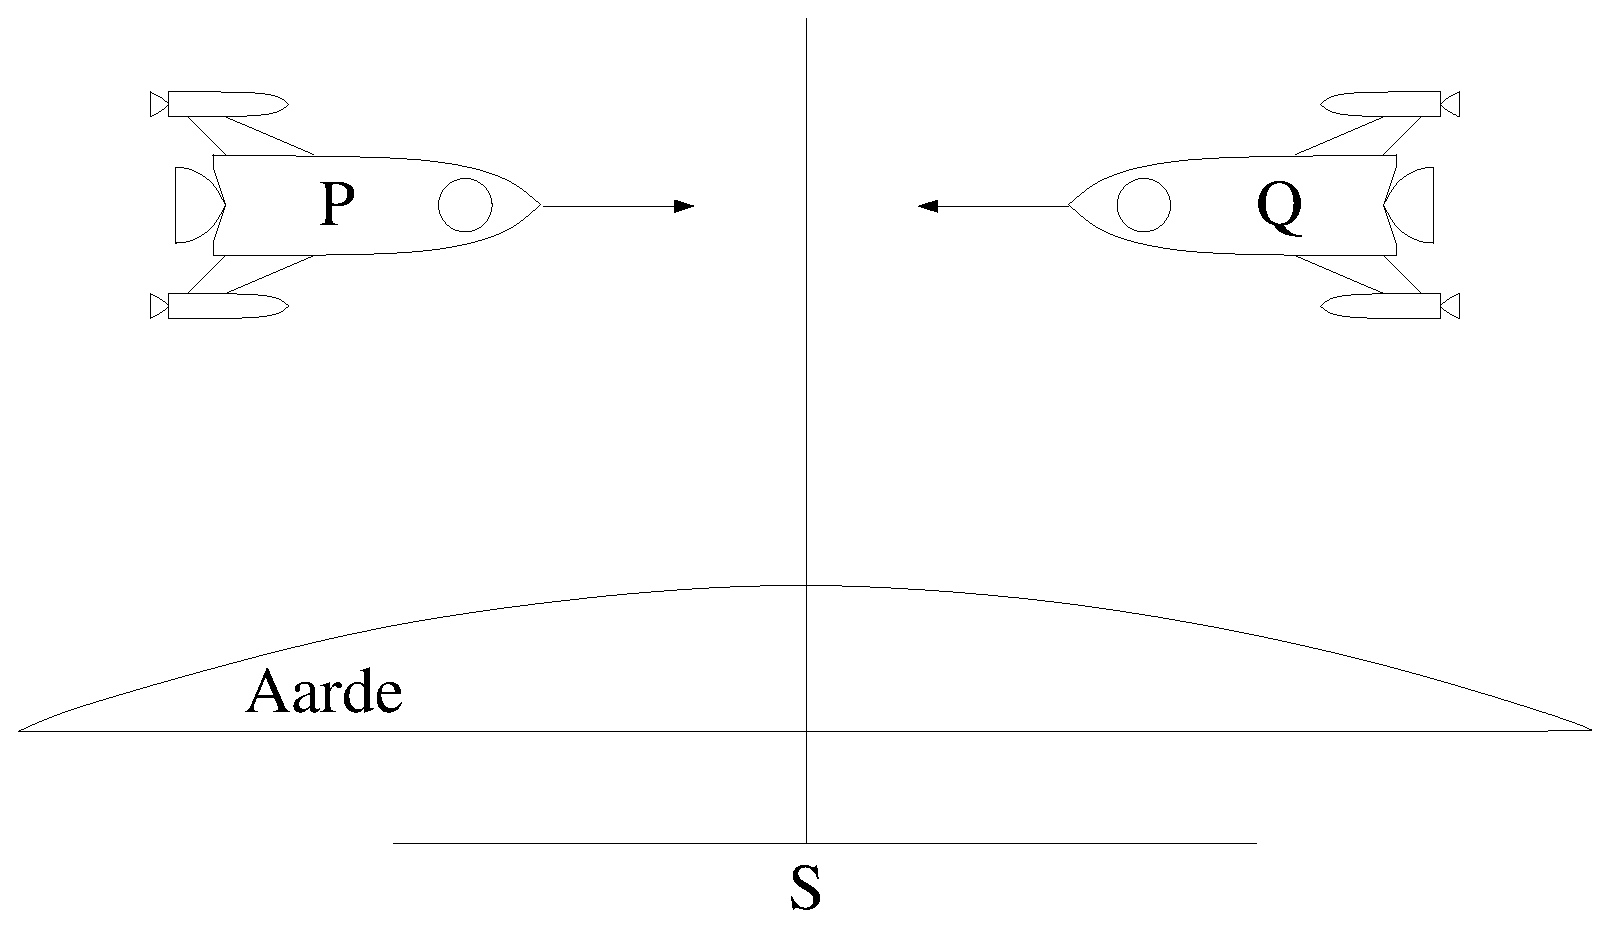
\includegraphics[width=.5\textwidth]{oefeningen.pictures/rockets}
\caption{Raketten}
\label{f:raket}
\end{figure}



Volgens  een waarnemer op aarde bevindt $Q$ zich op $t = 0$ op een afstand
$x = 4$ (lichtjaar), zodat $P$ 
en $Q$ elkaar in $x = 2$ (lichtjaar) zullen ontmoeten, na $t = 4$ jaar 
(dus $ct = 4$ lichtjaar). 
\begin{itemize}
\item [a.]
  Noteer  de  $x$-  en $ct$-co\"{o}rdinaten van de start van $P$,
de start van $Q$ en 
hun ontmoeting.
\end{itemize} 
We bekijken de gebeurtenis nu vanuit raketje $P$ (stelsel $S'$).
\begin{itemize}
\item [b.]
  Schrijf de Lorentztransformatie van $S$ naar $S'$ op (let op + en - tekens!)
\item [c.] 
  Vertaal  de  start  van $P$ en $Q$ en hun ontmoeting naar 
$S'$-co\"{o}rdinaten en noteer hiervan de $x'$- en $ct'$-co\"{o}rdinaten.
\item [d.]
  Welke  snelheid  $v' = \Delta x'/\Delta t'$ had raket $Q$, 
gezien vanuit $P$? 
Controleer dat met de snelheids-optelformule.
\end{itemize} 

%%%%%%%
\subsection{Lichtflitsen}
In een inertiaalsysteem $S$ worden in $A$ en $B$, $5$ $\mu$s na elkaar lichtflitsen uitgezonden.
De afstand $AB$ is $5$ km.
Als je in $S$ met een bepaalde snelheid $v$ parallel aan de lijn $AB$ beweegt, 
zie je de flitsen gelijktijdig.
Hoe groot moet $v$ zijn?


%%%%%%%
\subsection{Trein}
Een trein met een lengte $L_{0}$ (als hij stilstaat) davert langs een station
waarvan het perron een lengte $L < L_{0}$ heeft.
\begin{itemize}
\item [a.]
Hoe groot moet zijn snelheid zijn, zodat volgens iemand op het perron de staart
van de trein aan de achterkant van het perron is op hetzelfde moment als de kop van de trein aan de voorkant is?
\end{itemize}
Twee mensen aan de uiteinden van het perron slaan gelijktijdig 
(volgens hun eigen waarneming) een deuk in de trein.
\begin{itemize}
\item [b.]
Op welke afstand liggen die deuken uit elkaar volgens de mensen op het perron?
\item [c.]
En volgens de mensen in de rijdende trein?
\item [d.]
Waar zitten de deuken als de trein gestopt is?
\end{itemize}

%%%%%%%%%%%
%\subsection{Bewegende lichtklok}
%Ga na dat de lichtklok in figuur 4.2 op blz. 18 van de syllabus `tikt'
%als in formule 4.1 op blz. 17 van de syllabus.

